\title{Sparse neural networks of exclusive coincidence classes}
\author{Aleksander Mendoza}

\documentclass[12pt]{article}
\usepackage{tikz}
\usepackage[utf8]{inputenc}
\usepackage[T1]{fontenc}
\usepackage{lmodern}
\usepackage{amsfonts}
\usepackage{mathrsfs}
\usepackage{centernot}
\usepackage{listings}
\usepackage{mathtools}
\usepackage{xcolor}
\usepackage{amsthm}
\usepackage{amsmath}
\usepackage{amssymb}
\usepackage{tikzit}
\usepackage{enumitem}
\input{style.tikzstyles}
\DeclareMathOperator*{\argmax}{argmax}
\newtheorem{definition}{Definition}
\newtheorem{theorem}{Theorem}[section]
\newtheorem{corollary}{Corollary}[theorem]
\newtheorem{lemma}[theorem]{Lemma}
\renewcommand{\labelenumii}{\theenumii}
\renewcommand{\theenumii}{\theenumi.\arabic{enumii}.}
\begin{document}
\maketitle
\lstset{
	basicstyle=\ttfamily,
	mathescape
}


\begin{abstract}
We present a new model of neural networks that was inspired by an attempt to combine predictive coding and variational inference with sparse population coding and neural assembly calculus. This new approach can be used to learn extremely sparse and robust multi-layer networks without backpropagation or any error feedback whatsoever. It fits well with all biological constraints and leads to an emergence of receptive fields similar to those observed in neuroscience. It can be used to design biologically plausible convolutional networks without weight sharing. They are capable of extracting interdependent hierarchies of features, broadly similar to capsule networks proposed by Geoffrey Hinton.
\end{abstract} 


\section{Introduction}


Deep learning had its origins in an attempt to model biological neurons. Belief networks, Boltzmann and Helmholtz machines tried to capture the essence of neural computations using graphical models. A biological neuron could be interpreted as a node $f$ in some graph. Such nodes have binary values. When a neuron fires, the node holds value of $f=1$, otherwise it's $f=0$. Predictive coding and variational inference work on a higher level of abstraction and instead of modelling individual spikes, they focus on estimating the expectation $
\mathbb{E}(f)$, also known as firing rate. ECC networks operate on sparse populations and individual spikes.

\section{Exclusive coincidence classes}

Consider a binary vector $\boldsymbol{x}$. Every single bit $x_i$ represents certain observation, such as for example a pixel ($0=$white, $1=$black). Every possible configuration of bits in $\boldsymbol{x}$ has certain probability $p(\boldsymbol{x})$. Individual bits are often not independent of each other. Learning the joint probability $p(\boldsymbol{x})$ is challenging and often inefficient. That's why restricted Boltzmann machines are more practical than their unrestricted counterparts. Throughout the history of deep learning, the common trick was to assume that the bits independent anyway. Then consecutive deeper layers could reconstruct the interactions between inputs. Nonetheless, within the same layer of the neural network, the value of every neuron is computed independently of the others. 

We introduce a new and fundamentally different approach, called the exclusive coincidence classes (ECC). The data obtained by performing observations and measurements of the real world, often contains hidden structure, which introduces correlations of various features. Suppose there are $y_1,y_1...y_n$ distinct "events"
that may occur in the observed world and each of them manifests in its own way.
Going back to the example of $\boldsymbol{x}$ being pixels, we might image observing a straight metal bar. As we observe this bar rotate in front of our eyes, it will cast a line-shaped shadow on our retina. We might choose to treat different  rotations as distinct ``events'' and use $y_1...y_4$ to denote the angles $0^{\circ},45^{\circ},90^{\circ},135^{\circ}$ respectively. We can infer the rotation $\boldsymbol{y}$ from observations $\boldsymbol{x}$ by building a simple neural network with only a single densely connected linear layer. The training could be achieved using softmax and backpropagation. This is not what exclusive coincidence classes would do. 

Notice that all of the explanations $\boldsymbol{y}$ are mutually exclusive.
The bar cannot exist in two positions simultaneously. It could potentially lie somewhere in between angles $0^{\circ}$ and $45^{\circ}$, and then we might be tempted to proportionally assign some fractional values to $y_1$ and $y_2$. This  has been the dominant approach taken by the deep neural networks so far, but the biological neurons are noisy and unreliable. They could never operate with enough precision to pick up on such fractions. This is the reason why predictive coding has been forced to explain everything in terms of spike-rates $\mathbb{E}(f)$. This is also why deep networks are so brittle and allow for adversarial attacks. On the other hand, the biological neurons carry most of their information in individual spikes (the binary ``on'' bits) and sparse populations. When we restrict ourselves to only operate on binary values, then the explanations $\boldsymbol{y}$ must be mutually exclusive.

The connections between $\boldsymbol{x}$ and $\boldsymbol{y}$ could be represented using weight matrix $W$. In order to calculate the ``evidence'' accumulated for each explanation, we perform the product $\boldsymbol{x}W$.
Finally we assign $1$ to the $y_j$ which received the most ``evidence'' and all other $y$ are set to $0$. This is similar to the summation followed by threshold activation $y_j=f(\sum_{i}x_{i}w_{ji})$ in Rosenblatt's perceptron, except that here the neurons within a layer are not independent.

We can represent this mechanism in a graphical form, by introducing inhibitory neurons. All the excitatory neurons $\boldsymbol{y}$ are mutually-exclusive if they are connected to the same inhibitory neuron. Figure \ref{fig:graphical_models}
presents a comparison of all the existing types of graphical models. Boltzmann machines, Helmholtz machines, deep belief networks and deep neural networks etc. also fall into some of those categories. ECC networks do not belong there. They form their own ``orthogonal'' family of graphical models. 
\begin{figure}[!htbp]
	\centering
	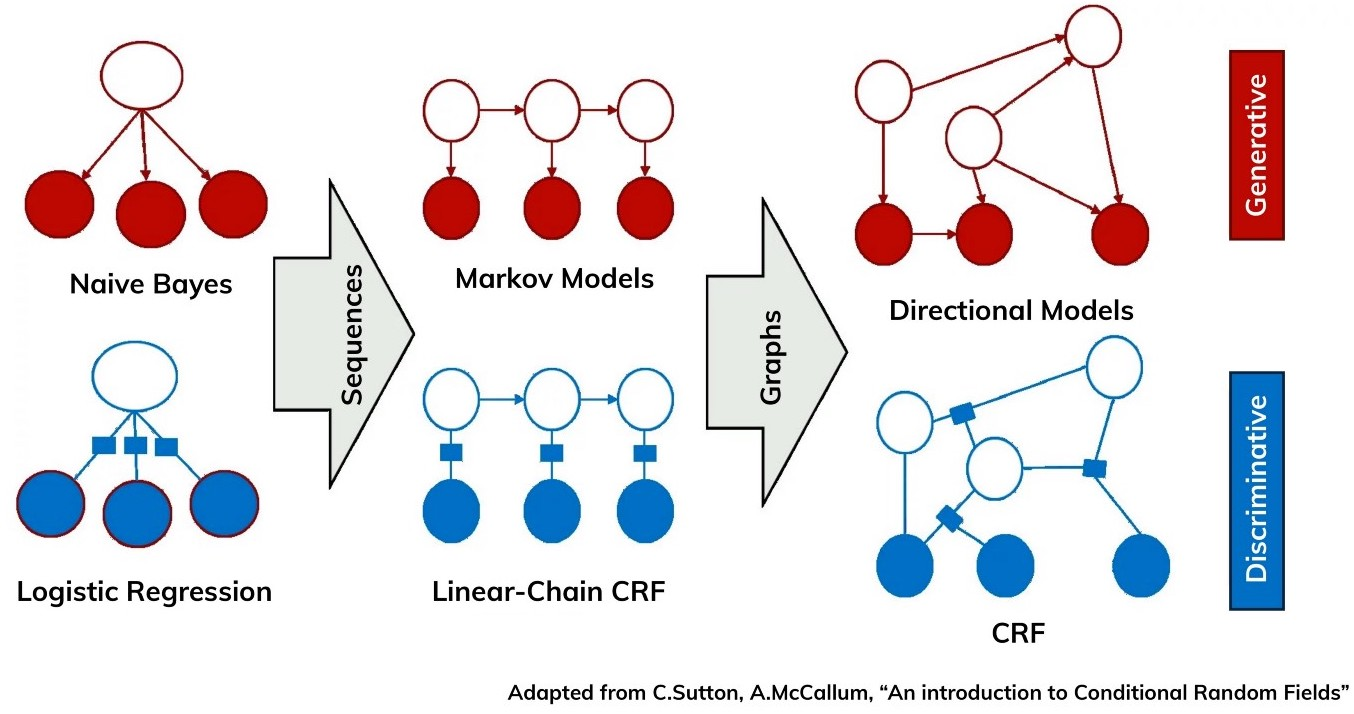
\includegraphics[width=14cm]{crf}
	\caption{Illustration presenting various families of graphical models. }
	\label{fig:graphical_models}
\end{figure} \\
Figure \ref{fig:ecc_graphical_models} presents an example of  ECC. 
\begin{figure}[!htbp]
	\centering
	
	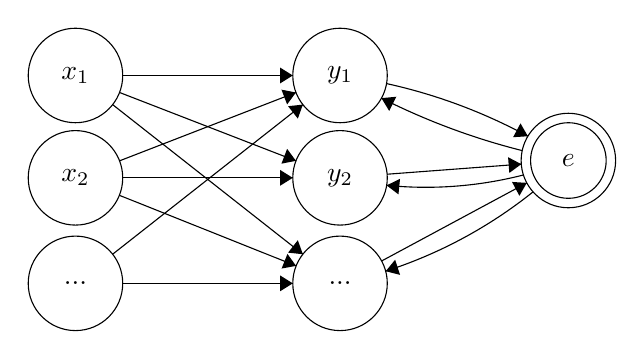
\begin{tikzpicture}[scale=0.2]
		\tikzstyle{every node}+=[inner sep=0pt]
		\draw [black] (40.1,-42.4) circle (3);
		\draw (40.1,-42.4) node {$e$};
		\draw [black] (40.1,-42.4) circle (2.4);
		\draw [black] (25.6,-37) circle (3);
		\draw (25.6,-37) node {$y_1$};
		\draw [black] (25.6,-43.5) circle (3);
		\draw (25.6,-43.5) node {$y_2$};
		\draw [black] (25.6,-50.2) circle (3);
		\draw (25.6,-50.2) node {$...$};
		\draw [black] (8.8,-37) circle (3);
		\draw (8.8,-37) node {$x_1$};
		\draw [black] (8.8,-43.5) circle (3);
		\draw (8.8,-43.5) node {$x_2$};
		\draw [black] (8.8,-50.2) circle (3);
		\draw (8.8,-50.2) node {$...$};
		\draw [black] (37.168,-41.77) arc (-104.11092:-116.74113:43.351);
		\fill [black] (28.23,-38.44) -- (28.72,-39.25) -- (29.17,-38.35);
		\draw [black] (37.246,-43.318) arc (-75.60821:-95.71526:24.95);
		\fill [black] (28.56,-43.98) -- (29.31,-44.55) -- (29.41,-43.56);
		\draw [black] (37.857,-44.391) arc (-51.32615:-72.11948:29.448);
		\fill [black] (28.5,-49.43) -- (29.41,-49.66) -- (29.1,-48.7);
		\draw [black] (11.8,-37) -- (22.6,-37);
		\fill [black] (22.6,-37) -- (21.8,-36.5) -- (21.8,-37.5);
		\draw [black] (11.6,-42.42) -- (22.8,-38.08);
		\fill [black] (22.8,-38.08) -- (21.88,-37.9) -- (22.24,-38.84);
		\draw [black] (11.16,-48.35) -- (23.24,-38.85);
		\fill [black] (23.24,-38.85) -- (22.3,-38.95) -- (22.92,-39.74);
		\draw [black] (11.6,-38.08) -- (22.8,-42.42);
		\fill [black] (22.8,-42.42) -- (22.24,-41.66) -- (21.88,-42.6);
		\draw [black] (11.16,-38.85) -- (23.24,-48.35);
		\fill [black] (23.24,-48.35) -- (22.92,-47.46) -- (22.3,-48.25);
		\draw [black] (11.8,-43.5) -- (22.6,-43.5);
		\fill [black] (22.6,-43.5) -- (21.8,-43) -- (21.8,-44);
		\draw [black] (11.8,-50.2) -- (22.6,-50.2);
		\fill [black] (22.6,-50.2) -- (21.8,-49.7) -- (21.8,-50.7);
		\draw [black] (11.59,-44.61) -- (22.81,-49.09);
		\fill [black] (22.81,-49.09) -- (22.26,-48.33) -- (21.89,-49.26);
		\draw [black] (28.555,-37.515) arc (77.60625:61.5417:34.266);
		\fill [black] (37.53,-40.86) -- (37.06,-40.04) -- (36.59,-40.92);
		\draw [black] (28.59,-43.27) -- (37.11,-42.63);
		\fill [black] (37.11,-42.63) -- (36.27,-42.19) -- (36.35,-43.19);
		\draw [black] (28.24,-48.78) -- (37.46,-43.82);
		\fill [black] (37.46,-43.82) -- (36.52,-43.76) -- (36.99,-44.64);
	\end{tikzpicture}
	\caption{An example of graphical model for exclusive coincidence classes. }
	\label{fig:ecc_graphical_models}
\end{figure}
The  $e$ node with double line represents an inhibitory neuron. All $y$ nodes are connected to it, meaning that they are mutually exclusive and only one of them can become active at the same time. All the excitatory $x$ nodes connected to any particular $y$ will contribute to its activation. The example above represents a bipartite graph, making it look like a feedforward network but in the more general case the directed connections could go both ways. The model does not need to be arranged in layers either.  

ECC are not trained using backpropagation. It is not even possible for two reasons. First is that binary values are not differentiable and second is that $\boldsymbol{y}$ are dependent on one another. Hebbian learning is necessary, but it is not sufficient. 

Suppose that observation $\boldsymbol{x}$ produces certain vector of evidence $\boldsymbol{s}=\boldsymbol{x}W$. The winning explanation $y_k=1$ is then selected using $k=argmax_j s_j$. The remaining explanations are inactive $y_j=0$ for all other $j\ne k$.
The hebbian learning tells us to strengthen $w_{ji}$ for all $i$ such that $x_i$ is active. Neurons in ECC networks work like coincidence detectors and their goal is to build stronger connections with those inputs that often occur together. The update rule is as follows
\[
w_{ik} := w_{ik} + \epsilon \text{ if } x_i=1
\]
where $\epsilon$ is some small learning rate that defines plasticity of the neuron. Different neurons could potentially use distinct $\epsilon$ values. In the real brain this is often affected by hormones. 

The hebbian rule above can only increment the weights. In order to prevent them from becoming too large, we follow this update by a normalization step.
\[
w_{ik} := \frac{w_{ik}}{ \sum_{ï} w_{ïk}} 
\]
As a result, the connections $w_{ik}$ that rarely drive activity of $y_k$ will gradually vanish. In the real brain, neurons cannot grow their dendrites indefinitely. Physical limits prevent them from making too many connections. Building a synapse to new input may come at the cost of losing other, less useful ones. Similarly, there is a limit to the neuron's activity. An individual neuron cannot fire all the time. We implement this limitation using the vector $\boldsymbol{a}$. Each neuron $y_j$ has a corresponding activity value $a_j$.
When $y_j$ fires, we decrement $a_j$ by a constant factor.
\[
a_j := a_j - \alpha \text{ if } y_j \text{ fired}
\]
Now we can include $\boldsymbol{a}$ in the computation of $k$.
\[\boldsymbol{s} = \boldsymbol{x}W \]
\[\boldsymbol{r} = \boldsymbol{s} + \boldsymbol{a} \]
\[k = \argmax_j r_j \]

All of the mechanisms presented so far are necessary. Without weight normalisation, the values would run off into infinity. The activity vector $\boldsymbol{a}$ allows for entropy maximisation. It ensures that all explanations
$\boldsymbol{y}$ self-organise in an optimal way. No $y$ should be able to dominate all others. Without $\boldsymbol{a}$, the network would produce trivial explanations by routing all activity to a single $y$ and leaving all others idle. By maximising entropy, we ensure that every $y$ carries plenty of information, that could be useful in higher layers.

The final algorithm looks as follows
\begin{lstlisting}
def infer(x,W,a,learning_enabled):
    s = x * W
    r = s + a
    k = argmax(r)
    if s[k] <= threshold:
        pass    // filter-out noise (optional)
    if learning_enabled:
        a[k] -= alpha
        W[:, k] += x * plasticity_constant[k]
        W[:, k] /= sum(W[:, k])
        // the W[:, k] notation stands for 
        // k-th column of a matrix
    return k
\end{lstlisting}

\iffalse
If we tried to use it on any data we would see that it struggles with building  any meaningful representations of data. Adding more layers would only lead to even worse performance. The problem is that ECC use two types of layers. What we have so far is only the ``convergent'' layer, but training will not work without adding ``separation'' layer. Consider the problem of modelling $\boldsymbol{x}\in\{[1,1,0],[0,1,1]\}$. We would like to assign these two vectors to different $y_1$ and $y_2$. A convergent layer will always try to generalise common information and it will notice that the two vectors share $\frac{1}{3}$ of their bits in common. As a result the layer will produce two almost identical weight vectors for both $y_1$ and $y_2$. Entropy maximisation will then cause the network to oscillate between the two explanations at random. To address this issue we need some mechanism to represent logical negations of features like $x_1\wedge \neg x_3$ and $\neg x_1\wedge x_3$. Such mechanism is called the pattern separation. 



In figure \ref{fig:ecc_graphical_models} every node $y$ sends input to the same $e$ and then $e$ inhibits all $y$. As a result all $y$ regulate themselves and each other. It is possible to build a graph like in figure \ref{fig:ecc_sep_graphical_models}, where these connections are not symmetric.
\begin{figure}[!htbp]
	\centering
	
	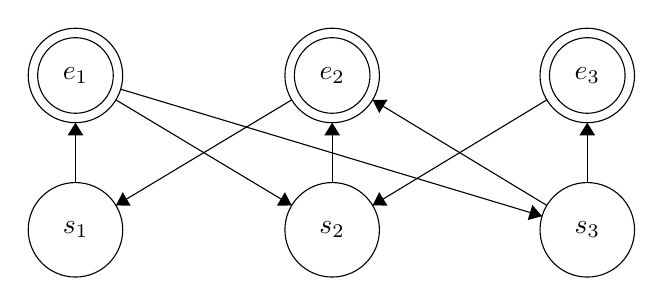
\begin{tikzpicture}[scale=0.2]
		
		\tikzstyle{every node}+=[inner sep=0pt]
		\draw [black] (7.2,-40.4) circle (3);
		\draw (7.2,-40.4) node {$e_1$};
		\draw [black] (7.2,-40.4) circle (2.4);
		\draw [black] (7.2,-50.2) circle (3);
		\draw (7.2,-50.2) node {$s_1$};
		\draw [black] (23.5,-50.2) circle (3);
		\draw (23.5,-50.2) node {$s_2$};
		\draw [black] (39.7,-50.2) circle (3);
		\draw (39.7,-50.2) node {$s_3$};
		\draw [black] (23.5,-40.4) circle (3);
		\draw (23.5,-40.4) node {$e_2$};
		\draw [black] (23.5,-40.4) circle (2.4);
		\draw [black] (39.7,-40.4) circle (3);
		\draw (39.7,-40.4) node {$e_3$};
		\draw [black] (39.7,-40.4) circle (2.4);
		\draw [black] (9.77,-41.95) -- (20.93,-48.65);
		\fill [black] (20.93,-48.65) -- (20.5,-47.81) -- (19.99,-48.67);
		\draw [black] (10.07,-41.27) -- (36.83,-49.33);
		\fill [black] (36.83,-49.33) -- (36.21,-48.62) -- (35.92,-49.58);
		\draw [black] (7.2,-47.2) -- (7.2,-43.4);
		\fill [black] (7.2,-43.4) -- (6.7,-44.2) -- (7.7,-44.2);
		\draw [black] (23.5,-47.2) -- (23.5,-43.4);
		\fill [black] (23.5,-43.4) -- (23,-44.2) -- (24,-44.2);
		\draw [black] (20.93,-41.95) -- (9.77,-48.65);
		\fill [black] (9.77,-48.65) -- (10.71,-48.67) -- (10.2,-47.81);
		\draw [black] (39.7,-47.2) -- (39.7,-43.4);
		\fill [black] (39.7,-43.4) -- (39.2,-44.2) -- (40.2,-44.2);
		\draw [black] (37.13,-48.65) -- (26.07,-41.95);
		\fill [black] (26.07,-41.95) -- (26.49,-42.79) -- (27.01,-41.94);
		\draw [black] (37.13,-41.95) -- (26.07,-48.65);
		\fill [black] (26.07,-48.65) -- (27.01,-48.66) -- (26.49,-47.81);
	\end{tikzpicture}
	\caption{Exclusive coincidence classes with asymmetric inhibition.}
	\label{fig:ecc_sep_graphical_models}
\end{figure}
 One excitatory neuron could drive inhibition of other excitatory neurons but not itself. Such a configuration allows the network to represent more sophisticated interactions between features, like $s_1\wedge\neg s_2 \wedge \neg s_3$,  $\neg s_1 \wedge s_2$ or $s_3\wedge\neg s_1 \wedge s_2$.  
 
Suppose that observations $\boldsymbol{x}$ are vectors of $n$ bits. In order to represent all possible conjunctions of negated and non-negated bits we would need to map $\boldsymbol{s}$ onto $2^n$ neurons in $\boldsymbol{y}$ layer. As we use sparse population coding,  we know that only a small fraction of bits in $\boldsymbol{x}$ will be active at any given time. Hence in practice it suffices to only use $\boldsymbol{y}$ of length $2n$ or a little less. We also do not need to keep individual inhibitory neurons in the memory. As the number of neurons increases, the effects of inhibition become approximately equivalent to choosing top $k$ highest activations. This $k$ is analogical to the top 1 best explanation in convergent layer. We will use bold $\boldsymbol{k}$ to denote a vector top $k$ elements $\boldsymbol{k}=[k_1,k2,...k_k]$ used in separation layer. 
The weights $W$ are sparse and initialised randomly. They do not need to be trained, because we do not intend to detect any coincidences (the plasticity $\epsilon$ is $0$). 
\fi

\section{Comparison of ECC and Bayesian/variational models}

Learning the joint probability $p(\boldsymbol{x})$ is a daunting task. Bayesian models, belief nets and deep neural networks build some graphical model and then factor out this distribution as
\[
p(\boldsymbol{x})=\prod_{y} p(\boldsymbol{y}|\pi(y))
\]
where $\pi(y)$ denotes parent/neighbours of $y$ in the graph. The convergent layers in ECC networks take a different approach and they model 
\[
p(\boldsymbol{x})=\sum_{j} p(\boldsymbol{x},y_j)
\]
We could say that the two approaches are ``orthogonal'' to each other.  While Bayesian and variational inference rely on independence of certain nodes $p(\boldsymbol{x})=p(x_1|\boldsymbol{y})p(x_2|\boldsymbol{y})...p(x_n|\boldsymbol{y})$, ECC try to partition $p(\boldsymbol{x})$ into mutually exclusive ``coincidence classes''
$p(\boldsymbol{x})=p(\boldsymbol{x},y_1)+p(\boldsymbol{x},y_2)+...+p(\boldsymbol{x},y_m)$. It could be seen as a linear combination of joint probability distributions
\[
p(\boldsymbol{x})=\sum_{j} p(\boldsymbol{x}|y_j) p(y_j)
\]
with the constraint that all coefficients $p(y_j)$ sum up to one $\sum_{j} p(y_j)=1$.
The ECC networks attempt to approximate this using the matrix $W$
\[
p(\boldsymbol{x})\approx \sum_{j} W_j p(y_j)
\]
where $W_j$ is the $j^{th}$ column of $W$. We could think of $p(\boldsymbol{x}|y_j)$ as ``eigendistributions''. Then ECC networks learn by performing ``eigendecomposition'' of $p(\boldsymbol{x})$. The challenge here lies in the fact that such eigendecomposition of joint distributions is an ill-defined problem. There might exist infinitely many coefficients (summed under Lebesgue integral)
\[
p(\boldsymbol{x})= \int_y p(\boldsymbol{x}|y) p(y)
\]
Most of those coefficients would be very small. We are hoping to approximate $p(\boldsymbol{x})$ with only a finite number of them. We could draw an analogy to data compression algorithms, where we try to ``compress'' $p(\boldsymbol{x})$ by only keeping the $m$ largest eigenvalues and truncating all the rest. The only difference here is that the ``compression'' is loss-less. The probability must sum up to one. If we truncated any of the eigendistributions,  this property would be violated. Instead we can add some of the eigendistributions together. For example a linear combination of $3$ components
\[
p(\boldsymbol{x}|y_1) p(y_1)+p(\boldsymbol{x}|y_2) p(y_2)+p(\boldsymbol{x}|y_3) p(y_3)
\]
could be rewritten using only $2$ components
\[
p(\boldsymbol{x}|y_1) p(y_1)+p(\boldsymbol{x}|y_2\text{ or }y_3) (p(y_2)+p(y_3))
\]
The ECC networks are not capable of precisely capturing the distribution $p(\boldsymbol{x}|y_2\text{ or }y_3)$, because using a weight matrix $W$ requires independence of all $x$ variables
\[
p(\boldsymbol{x}|y_j) = p(x_1|y_j)p(x_2|y_j)...p(x_n|y_j) = \boldsymbol{x} W_j
\]
which is not always true. We can only approximate $p(\boldsymbol{x}|y_2\text{ or }y_3)$
using the combination
\[
p(\boldsymbol{x}|y_2\text{ or }y_3) p(y_2\text{ or }y_3)= p(\boldsymbol{x}|y_2) p(y_2)+p(\boldsymbol{x}|y_3) p(y_3) \approx \boldsymbol{x}W_2p(y_2) + \boldsymbol{x}W_3 p(y_3)
\]
under the assumption that $p(y_3)$ is a much smaller eigenvalue than $p(y_2)$.
The above approximation would be an exact equality only in a special case, where the two eigendistributions are congruent (equal up to a constant):
\[p(\boldsymbol{x},y_3)=C p(\boldsymbol{x},y_2)\]
In practice it is unlikely that we could find such congruences, but the more similar the two summed distributions are, the more precise our approximation of $p(\boldsymbol{x})$ would be.
Learning is the matter of clustering the eigendistributions by their similarity and then summing up all the elements within the same cluster to obtain the final approximation. If we had only a finite number of observations $\boldsymbol{x}$, then we could find an optimal solution to this problem.
A more interesting case is when we attempt to do online learning with possibly infinite stream of new observations. Then we need an iterative algorithm and this is exactly what ECC networks are. 


As we have established so far, our goal is to find $m$ most significant eigenvalues. It makes little sense to model latent causes $y$ that are significantly less likely than the rest. Hence we perform entropy maximisation using activity vector $\boldsymbol{a}$. The entropy
\[
H(\boldsymbol{y}) = - \sum_{j=1}^{m}p(y_j)\log p(y_j)
\]
has its highest value, when all $p(y)$ are approximately equal
\[
p(y_1)\approx p(y_2)\approx...\approx p(y_m)
\]
When this holds, then we can simplify the learned model to
\[
p(\boldsymbol{x}) \approx \sum_{j=1}^{m}\boldsymbol{x}W_jp(y_j) \approx \frac{\sum_{j=1}^{m}\boldsymbol{x}W_j}{m}
\]

Because we are only interested in capturing the eigendistributions with highest probabilities, the networks will learn to recognise only the most general and frequent patterns. They can't overfit to training data and the concept of adversarial examples does not exist here. They could also generalise to new environments with ease, because many novel distribution could be expressed as linear combinations of the same fundamental eigendistributions but with different coefficients. The ECC networks have all the characteristics necessary to implement general human-like AI that learns any task with a few shots, as long as the novel observation can be encoded using some conjunction of simpler features.

One very important property should be noted. Whenever a new observation $\boldsymbol{x}$ is received, we attempt to find the best matching cluster $k=\argmax_j r_j$. If the learned model is optimal, then the expected value $\mathbb{E}(s_k)$ of best-matching $s_k$ is going to be maximised. Empirically it can indeed be confirmed that $\mathbb{E}(s_k)$ always increases and eventually converges on some high value.




\section{Exclusive coincidence machine}

In this section we introduce the final working model of a network that can build meaningful receptive fields. A receptive field is defined as probability distribution over the set of all possible vectors $\boldsymbol{x}$. It tells us how likely a given observation vector is to activate a specific $y_j$. Each $y_j$ has its own receptive field. Such probability distribution $p(\boldsymbol{x}|y_j)$ is also referred to as ``coincidence class'' or ``eigendistribution''. 

In general case the topology of an ECC network might be chaotic and highly recurrent. We distinguish a special subset of networks, known as ECC machines. Their topologies are restricted to always be arranged in a strictly layered form (multipartite graph). Figure \ref{fig:ecc_machine} shows a general schematic of a multilayer ECC machine. 
\begin{figure}[!htbp]
	\centering

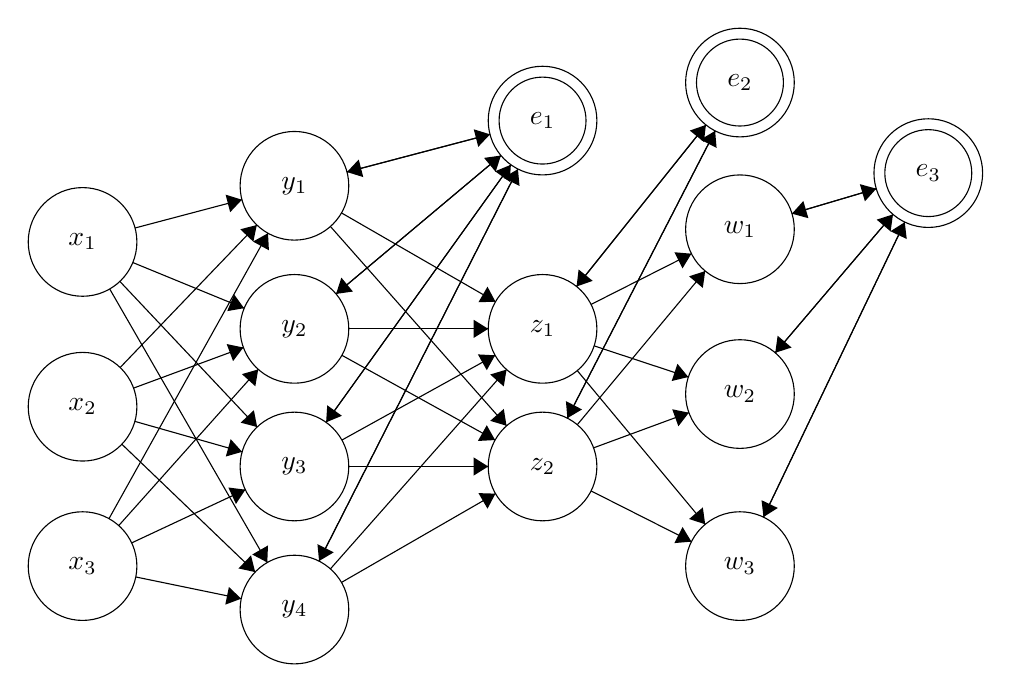
\begin{tikzpicture}[scale=0.23]
	\tikzstyle{every node}+=[inner sep=0pt]
	\draw [black] (10,-11.9) circle (3);
	\draw (10,-11.9) node {$x_1$};
	\draw [black] (10,-21) circle (3);
	\draw (10,-21) node {$x_2$};
	\draw [black] (10,-29.8) circle (3);
	\draw (10,-29.8) node {$x_3$};
	\draw [black] (21.7,-8.8) circle (3);
	\draw (21.7,-8.8) node {$y_1$};
	\draw [black] (21.7,-16.7) circle (3);
	\draw (21.7,-16.7) node {$y_2$};
	\draw [black] (21.7,-24.3) circle (3);
	\draw (21.7,-24.3) node {$y_3$};
	\draw [black] (21.7,-32.2) circle (3);
	\draw (21.7,-32.2) node {$y_4$};
	\draw [black] (35.4,-16.7) circle (3);
	\draw (35.4,-16.7) node {$z_1$};
	\draw [black] (35.4,-24.3) circle (3);
	\draw (35.4,-24.3) node {$z_2$};
	\draw [black] (46.3,-11.2) circle (3);
	\draw (46.3,-11.2) node {$w_1$};
	\draw [black] (46.3,-20.3) circle (3);
	\draw (46.3,-20.3) node {$w_2$};
	\draw [black] (46.3,-29.8) circle (3);
	\draw (46.3,-29.8) node {$w_3$};
	\draw [black] (35.4,-5.2) circle (3);
	\draw (35.4,-5.2) node {$e_1$};
	\draw [black] (35.4,-5.2) circle (2.4);
	\draw [black] (46.3,-3.1) circle (3);
	\draw (46.3,-3.1) node {$e_2$};
	\draw [black] (46.3,-3.1) circle (2.4);
	\draw [black] (56.7,-8.1) circle (3);
	\draw (56.7,-8.1) node {$e_3$};
	\draw [black] (56.7,-8.1) circle (2.4);
	\draw [black] (12.9,-11.13) -- (18.8,-9.57);
	\fill [black] (18.8,-9.57) -- (17.9,-9.29) -- (18.15,-10.26);
	\draw [black] (12.78,-13.04) -- (18.92,-15.56);
	\fill [black] (18.92,-15.56) -- (18.37,-14.8) -- (17.99,-15.72);
	\draw [black] (12.82,-19.97) -- (18.88,-17.73);
	\fill [black] (18.88,-17.73) -- (17.96,-17.54) -- (18.31,-18.48);
	\draw [black] (12.06,-14.08) -- (19.64,-22.12);
	\fill [black] (19.64,-22.12) -- (19.46,-21.19) -- (18.73,-21.88);
	\draw [black] (11.5,-14.5) -- (20.2,-29.6);
	\fill [black] (20.2,-29.6) -- (20.24,-28.66) -- (19.37,-29.16);
	\draw [black] (12,-27.56) -- (19.7,-18.94);
	\fill [black] (19.7,-18.94) -- (18.8,-19.2) -- (19.54,-19.87);
	\draw [black] (12.71,-28.52) -- (18.99,-25.58);
	\fill [black] (18.99,-25.58) -- (18.05,-25.46) -- (18.47,-26.37);
	\draw [black] (12.94,-30.4) -- (18.76,-31.6);
	\fill [black] (18.76,-31.6) -- (18.08,-30.95) -- (17.88,-31.93);
	\draw [black] (12.08,-18.83) -- (19.62,-10.97);
	\fill [black] (19.62,-10.97) -- (18.71,-11.2) -- (19.43,-11.89);
	\draw [black] (12.89,-21.81) -- (18.81,-23.49);
	\fill [black] (18.81,-23.49) -- (18.18,-22.79) -- (17.91,-23.75);
	\draw [black] (12.17,-23.07) -- (19.53,-30.13);
	\fill [black] (19.53,-30.13) -- (19.3,-29.21) -- (18.61,-29.93);
	\draw [black] (11.46,-27.18) -- (20.24,-11.42);
	\fill [black] (20.24,-11.42) -- (19.41,-11.88) -- (20.29,-12.36);
	\draw [black] (24.3,-10.3) -- (32.8,-15.2);
	\fill [black] (32.8,-15.2) -- (32.36,-14.37) -- (31.86,-15.23);
	\draw [black] (24.7,-16.7) -- (32.4,-16.7);
	\fill [black] (32.4,-16.7) -- (31.6,-16.2) -- (31.6,-17.2);
	\draw [black] (24.32,-22.84) -- (32.78,-18.16);
	\fill [black] (32.78,-18.16) -- (31.83,-18.11) -- (32.32,-18.98);
	\draw [black] (24.3,-30.7) -- (32.8,-25.8);
	\fill [black] (32.8,-25.8) -- (31.86,-25.77) -- (32.36,-26.63);
	\draw [black] (23.69,-11.05) -- (33.41,-22.05);
	\fill [black] (33.41,-22.05) -- (33.26,-21.12) -- (32.51,-21.78);
	\draw [black] (24.32,-18.16) -- (32.78,-22.84);
	\fill [black] (32.78,-22.84) -- (32.32,-22.02) -- (31.83,-22.89);
	\draw [black] (23.69,-29.95) -- (33.41,-18.95);
	\fill [black] (33.41,-18.95) -- (32.51,-19.22) -- (33.26,-19.88);
	\draw [black] (24.7,-24.3) -- (32.4,-24.3);
	\fill [black] (32.4,-24.3) -- (31.6,-23.8) -- (31.6,-24.8);
	\draw [black] (38.08,-15.35) -- (43.62,-12.55);
	\fill [black] (43.62,-12.55) -- (42.68,-12.47) -- (43.13,-13.36);
	\draw [black] (38.25,-17.64) -- (43.45,-19.36);
	\fill [black] (43.45,-19.36) -- (42.85,-18.63) -- (42.53,-19.58);
	\draw [black] (38.22,-23.27) -- (43.48,-21.33);
	\fill [black] (43.48,-21.33) -- (42.56,-21.14) -- (42.9,-22.08);
	\draw [black] (38.08,-25.65) -- (43.62,-28.45);
	\fill [black] (43.62,-28.45) -- (43.13,-27.64) -- (42.68,-28.53);
	\draw [black] (37.32,-21.99) -- (44.38,-13.51);
	\fill [black] (44.38,-13.51) -- (43.49,-13.8) -- (44.25,-14.44);
	\draw [black] (37.32,-19.01) -- (44.38,-27.49);
	\fill [black] (44.38,-27.49) -- (44.25,-26.56) -- (43.49,-27.2);
	\draw [black] (32.5,-5.96) -- (24.6,-8.04);
	\fill [black] (24.6,-8.04) -- (25.5,-8.32) -- (25.25,-7.35);
	\draw [black] (24.6,-8.04) -- (32.5,-5.96);
	\fill [black] (32.5,-5.96) -- (31.6,-5.68) -- (31.85,-6.65);
	\draw [black] (33.1,-7.13) -- (24,-14.77);
	\fill [black] (24,-14.77) -- (24.93,-14.64) -- (24.29,-13.87);
	\draw [black] (24,-14.77) -- (33.1,-7.13);
	\fill [black] (33.1,-7.13) -- (32.17,-7.26) -- (32.81,-8.03);
	\draw [black] (33.65,-7.64) -- (23.45,-21.86);
	\fill [black] (23.45,-21.86) -- (24.32,-21.5) -- (23.51,-20.92);
	\draw [black] (23.45,-21.86) -- (33.65,-7.64);
	\fill [black] (33.65,-7.64) -- (32.78,-8) -- (33.59,-8.58);
	\draw [black] (23.06,-29.52) -- (34.04,-7.88);
	\fill [black] (34.04,-7.88) -- (33.23,-8.36) -- (34.13,-8.81);
	\draw [black] (34.04,-7.88) -- (23.06,-29.52);
	\fill [black] (23.06,-29.52) -- (23.87,-29.04) -- (22.97,-28.59);
	\draw [black] (37.28,-14.36) -- (44.42,-5.44);
	\fill [black] (44.42,-5.44) -- (43.53,-5.75) -- (44.31,-6.38);
	\draw [black] (36.77,-21.63) -- (44.93,-5.77);
	\fill [black] (44.93,-5.77) -- (44.12,-6.25) -- (45.01,-6.71);
	\draw [black] (44.42,-5.44) -- (37.28,-14.36);
	\fill [black] (37.28,-14.36) -- (38.17,-14.05) -- (37.39,-13.42);
	\draw [black] (44.93,-5.77) -- (36.77,-21.63);
	\fill [black] (36.77,-21.63) -- (37.58,-21.15) -- (36.69,-20.69);
	\draw [black] (53.83,-8.96) -- (49.17,-10.34);
	\fill [black] (49.17,-10.34) -- (50.08,-10.59) -- (49.8,-9.64);
	\draw [black] (49.17,-10.34) -- (53.83,-8.96);
	\fill [black] (53.83,-8.96) -- (52.92,-8.71) -- (53.2,-9.66);
	\draw [black] (48.25,-18.02) -- (54.75,-10.38);
	\fill [black] (54.75,-10.38) -- (53.85,-10.67) -- (54.62,-11.32);
	\draw [black] (54.75,-10.38) -- (48.25,-18.02);
	\fill [black] (48.25,-18.02) -- (49.15,-17.73) -- (48.38,-17.08);
	\draw [black] (47.6,-27.09) -- (55.4,-10.81);
	\fill [black] (55.4,-10.81) -- (54.61,-11.31) -- (55.51,-11.74);
	\draw [black] (55.4,-10.81) -- (47.6,-27.09);
	\fill [black] (47.6,-27.09) -- (48.39,-26.59) -- (47.49,-26.16);
\end{tikzpicture}
	\caption{Exclusive coincidence machine}
	\label{fig:ecc_machine}
\end{figure} 
Such networks can be easily formalised and efficiently implemented. The fundamental building blocks are populations and weight matrices. A population is defined as tuple $(\boldsymbol{a},\boldsymbol{s})$
It is possible to arrange the topology to resemble convolutional neural networks.
Imagine taking several copies of the network from figure \ref{fig:ecc_machine} and stacking them next to each other in such a way that each one sees only a small patch of the input image. Figure \ref{fig:ecc_conv_machine} presents an example of one-dimensional convolution. 
\begin{figure}[!htbp]
	\centering

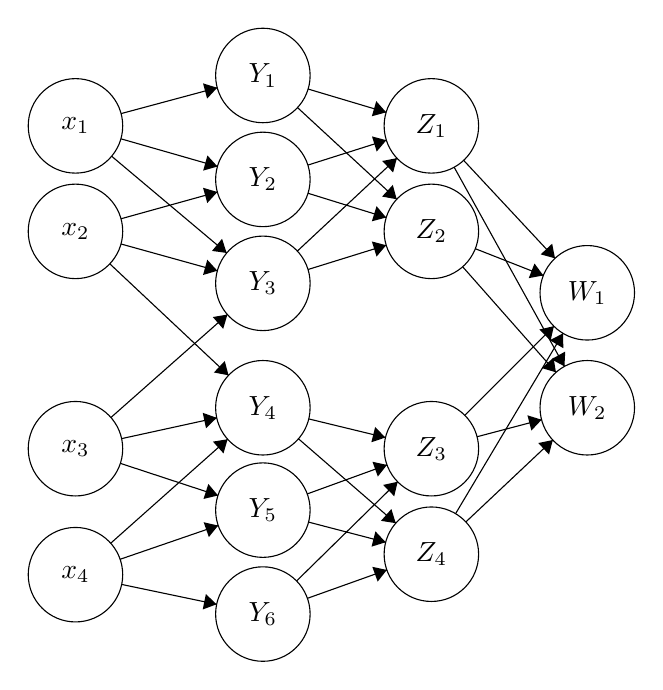
\begin{tikzpicture}[scale=0.2]
	\tikzstyle{every node}+=[inner sep=0pt]
	\draw [black] (21.9,-22.4) circle (3);
	\draw (21.9,-22.4) node {$Y_1$};
	\draw [black] (21.9,-29) circle (3);
	\draw (21.9,-29) node {$Y_2$};
	\draw [black] (21.9,-35.6) circle (3);
	\draw (21.9,-35.6) node {$Y_3$};
	\draw [black] (10,-25.6) circle (3);
	\draw (10,-25.6) node {$x_1$};
	\draw [black] (10,-32.3) circle (3);
	\draw (10,-32.3) node {$x_2$};
	\draw [black] (10,-46.1) circle (3);
	\draw (10,-46.1) node {$x_3$};
	\draw [black] (21.9,-43.5) circle (3);
	\draw (21.9,-43.5) node {$Y_4$};
	\draw [black] (32.6,-25.6) circle (3);
	\draw (32.6,-25.6) node {$Z_1$};
	\draw [black] (32.6,-32.3) circle (3);
	\draw (32.6,-32.3) node {$Z_2$};
	\draw [black] (42.5,-36.2) circle (3);
	\draw (42.5,-36.2) node {$W_1$};
	\draw [black] (42.5,-43.5) circle (3);
	\draw (42.5,-43.5) node {$W_2$};
	\draw [black] (10,-54.1) circle (3);
	\draw (10,-54.1) node {$x_4$};
	\draw [black] (21.9,-50) circle (3);
	\draw (21.9,-50) node {$Y_5$};
	\draw [black] (32.6,-46.1) circle (3);
	\draw (32.6,-46.1) node {$Z_3$};
	\draw [black] (32.6,-52.8) circle (3);
	\draw (32.6,-52.8) node {$Z_4$};
	\draw [black] (21.9,-56.6) circle (3);
	\draw (21.9,-56.6) node {$Y_6$};
	\draw [black] (12.9,-24.82) -- (19,-23.18);
	\fill [black] (19,-23.18) -- (18.1,-22.9) -- (18.36,-23.87);
	\draw [black] (12.88,-26.42) -- (19.02,-28.18);
	\fill [black] (19.02,-28.18) -- (18.38,-27.48) -- (18.11,-28.44);
	\draw [black] (24.77,-23.26) -- (29.73,-24.74);
	\fill [black] (29.73,-24.74) -- (29.1,-24.03) -- (28.82,-24.99);
	\draw [black] (24.1,-24.44) -- (30.4,-30.26);
	\fill [black] (30.4,-30.26) -- (30.15,-29.35) -- (29.47,-30.09);
	\draw [black] (24.76,-28.09) -- (29.74,-26.51);
	\fill [black] (29.74,-26.51) -- (28.83,-26.27) -- (29.13,-27.23);
	\draw [black] (24.09,-33.55) -- (30.41,-27.65);
	\fill [black] (30.41,-27.65) -- (29.48,-27.83) -- (30.17,-28.56);
	\draw [black] (24.77,-34.72) -- (29.73,-33.18);
	\fill [black] (29.73,-33.18) -- (28.82,-32.94) -- (29.12,-33.9);
	\draw [black] (34.65,-27.79) -- (40.45,-34.01);
	\fill [black] (40.45,-34.01) -- (40.27,-33.08) -- (39.54,-33.76);
	\draw [black] (34.05,-28.23) -- (41.05,-40.87);
	\fill [black] (41.05,-40.87) -- (41.1,-39.93) -- (40.22,-40.42);
	\draw [black] (35.39,-33.4) -- (39.71,-35.1);
	\fill [black] (39.71,-35.1) -- (39.15,-34.34) -- (38.78,-35.27);
	\draw [black] (34.59,-34.55) -- (40.51,-41.25);
	\fill [black] (40.51,-41.25) -- (40.36,-40.32) -- (39.61,-40.98);
	\draw [black] (12.89,-33.1) -- (19.01,-34.8);
	\fill [black] (19.01,-34.8) -- (18.37,-34.1) -- (18.1,-35.07);
	\draw [black] (12.85,-47.03) -- (19.05,-49.07);
	\fill [black] (19.05,-49.07) -- (18.44,-48.34) -- (18.13,-49.29);
	\draw [black] (12.24,-52.1) -- (19.66,-45.5);
	\fill [black] (19.66,-45.5) -- (18.73,-45.65) -- (19.4,-46.4);
	\draw [black] (12.84,-53.12) -- (19.06,-50.98);
	\fill [black] (19.06,-50.98) -- (18.14,-50.77) -- (18.47,-51.71);
	\draw [black] (24.82,-44.21) -- (29.68,-45.39);
	\fill [black] (29.68,-45.39) -- (29.03,-44.72) -- (28.79,-45.69);
	\draw [black] (24.16,-45.47) -- (30.34,-50.83);
	\fill [black] (30.34,-50.83) -- (30.06,-49.93) -- (29.4,-50.68);
	\draw [black] (24.8,-50.76) -- (29.7,-52.04);
	\fill [black] (29.7,-52.04) -- (29.05,-51.35) -- (28.8,-52.32);
	\draw [black] (12.94,-54.72) -- (18.96,-55.98);
	\fill [black] (18.96,-55.98) -- (18.28,-55.33) -- (18.08,-56.31);
	\draw [black] (24.73,-55.6) -- (29.77,-53.8);
	\fill [black] (29.77,-53.8) -- (28.85,-53.6) -- (29.19,-54.54);
	\draw [black] (24.72,-48.97) -- (29.78,-47.13);
	\fill [black] (29.78,-47.13) -- (28.86,-46.93) -- (29.2,-47.87);
	\draw [black] (24.04,-54.5) -- (30.46,-48.2);
	\fill [black] (30.46,-48.2) -- (29.54,-48.4) -- (30.24,-49.12);
	\draw [black] (35.5,-45.34) -- (39.6,-44.26);
	\fill [black] (39.6,-44.26) -- (38.7,-43.98) -- (38.95,-44.95);
	\draw [black] (34.79,-50.75) -- (40.31,-45.55);
	\fill [black] (40.31,-45.55) -- (39.39,-45.74) -- (40.07,-46.47);
	\draw [black] (34.72,-43.98) -- (40.38,-38.32);
	\fill [black] (40.38,-38.32) -- (39.46,-38.53) -- (40.17,-39.24);
	\draw [black] (34.14,-50.22) -- (40.96,-38.78);
	\fill [black] (40.96,-38.78) -- (40.12,-39.21) -- (40.98,-39.72);
	\draw [black] (12.18,-34.36) -- (19.72,-41.44);
	\fill [black] (19.72,-41.44) -- (19.48,-40.53) -- (18.79,-41.26);
	\draw [black] (12.25,-44.12) -- (19.65,-37.58);
	\fill [black] (19.65,-37.58) -- (18.72,-37.74) -- (19.38,-38.49);
	\draw [black] (12.89,-31.5) -- (19.01,-29.8);
	\fill [black] (19.01,-29.8) -- (18.1,-29.53) -- (18.37,-30.5);
	\draw [black] (12.93,-45.46) -- (18.97,-44.14);
	\fill [black] (18.97,-44.14) -- (18.08,-43.82) -- (18.29,-44.8);
	\draw [black] (12.3,-27.53) -- (19.6,-33.67);
	\fill [black] (19.6,-33.67) -- (19.31,-32.77) -- (18.67,-33.54);
	\draw [black] (24.77,-29.88) -- (29.73,-31.42);
	\fill [black] (29.73,-31.42) -- (29.12,-30.7) -- (28.82,-31.66);
\end{tikzpicture}
	\caption{Convolutional exclusive coincidence machine}
	\label{fig:ecc_conv_machine}
\end{figure} 
The neuron $y_1$ can ``see'' input coming from $x_1,x_2$ and $x_3$. We say that the topological receptive field $\tau$ of $y_1$ is $\tau(y_1)=\{1,2, 3\}$. Both $y_1$ and $y_2$ have the same or almost the same $\tau$ to each other but significantly differ from $y_3$ and $y_4$. We could say that $y_1,y_2$ form one column, whereas $y_3,y_4$ form another. The $\boldsymbol{z}$ combines  information from both columns and builds coarser, more general, coincidence classes. The receptive topology is the driving force behind receptive fields.
If the probability distribution $p(x_1,x_2,x_3)$ is the same as that of $p(x_3,x_4,x_5)$, then $y_1,y_2$ will develop similar receptive fields to those of $y_3,y_4$. There is not need for weight sharing. The network will always self-organise optimally. 

This model achieves exactly what Geoffrey Hinton's capsule networks were originally meant to do. Even though $p(x_1,x_2,x_3)=p(x_3,x_4,x_5)$, the neurons 
 $y_1,y_2$  are not equivalent to $y_3,y_4$. They recognise the same signal but at different locations. The $\boldsymbol{z}$ then has access to such location-carrying information and builds hierarchies of features that account for their spacial relationships. 

\section{Experiments}

We built a 4 layer ECC network and trained it without any labels and using nothing more than Hebbian learning rules. Figure \ref{fig:experiment4} presents receptive fields of neurons from layer 4 in randomly initialised network before training and the exclusive coincidence classes that emerge after enough iterations. Figure \ref{fig:experiment3} represents neurons from one column in layer 3 after training.
At the beginning the receptive fields tend to fluctuate. Their shapes appear blurry and random. After enough iterations, the receptive fields stabilise and converge to much sharper and more detailed shapes. The training was performed by taking random 11x11 patches of MNIST images. Before and after training, the receptive fields were evaluated on a different set of  unseen patches. Hence it can be seen that the network does not merely cluster
the observed data, but instead it forms robust classes of features that generalise well.

\begin{figure}[!htbp]
	\centering
	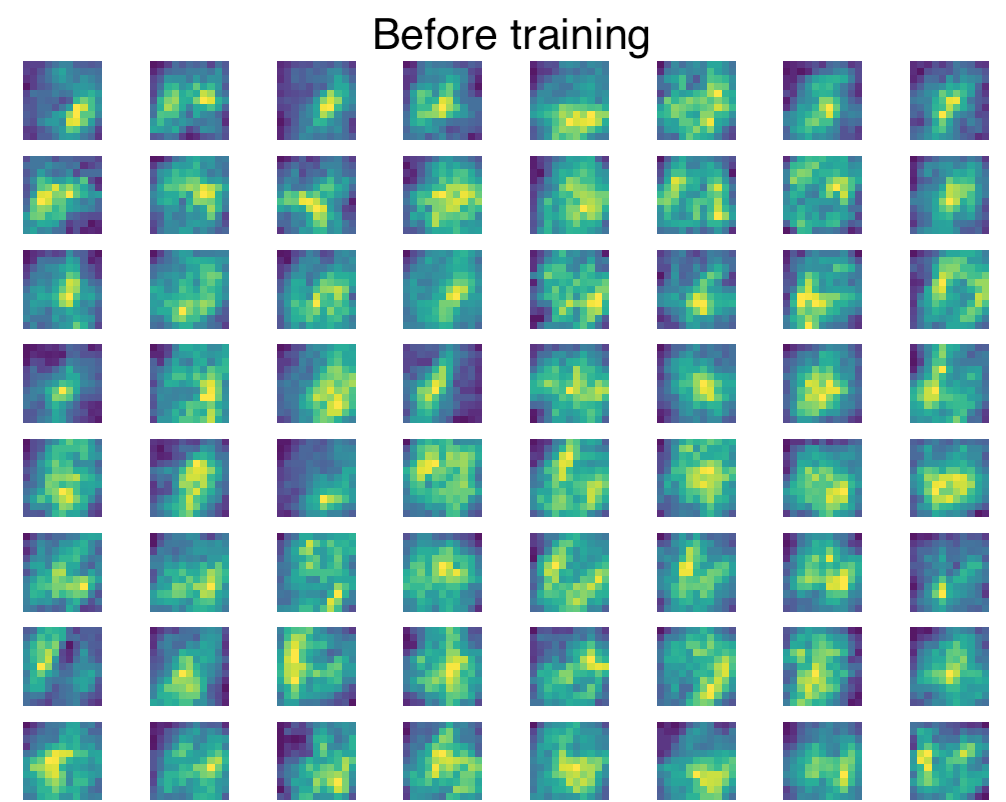
\includegraphics[width=11cm]{predictive_coding_stacked2_experiment4 before}
	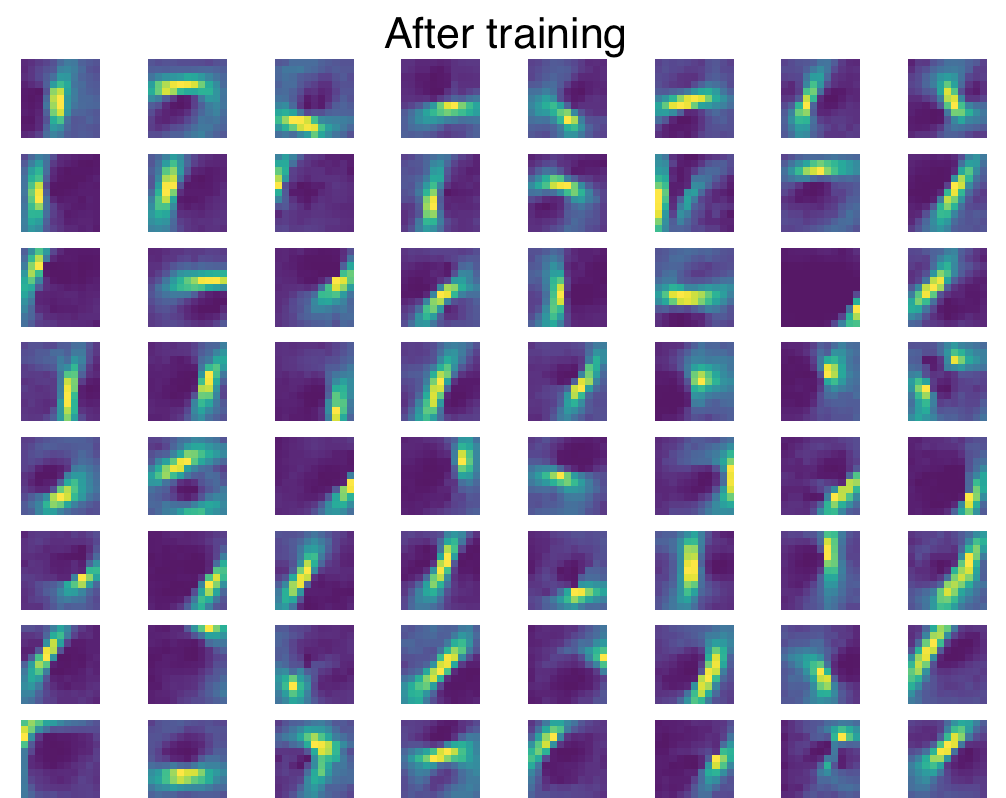
\includegraphics[width=11cm]{predictive_coding_stacked2_experiment4 after}
	\caption{Receptive fields of 64 neurons in the fourth layer}
	\label{fig:experiment4}
\end{figure} 

\begin{figure}[!htbp]
	\centering
	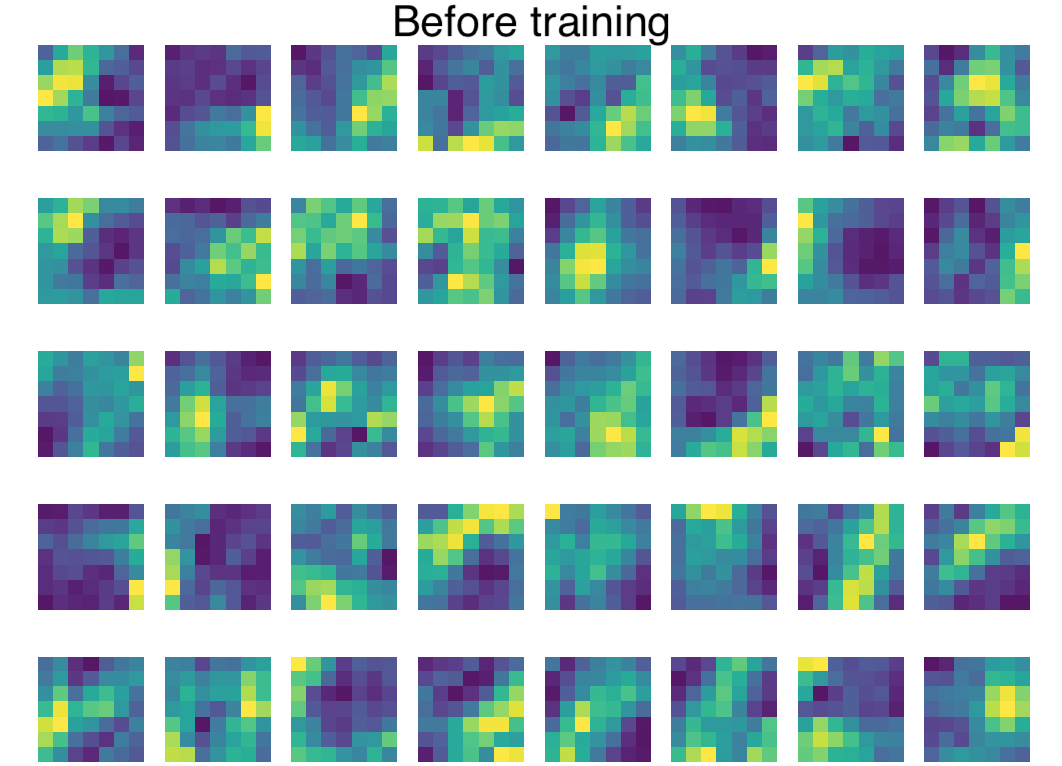
\includegraphics[width=12cm]{predictive_coding_stacked2_experiment3 before}
	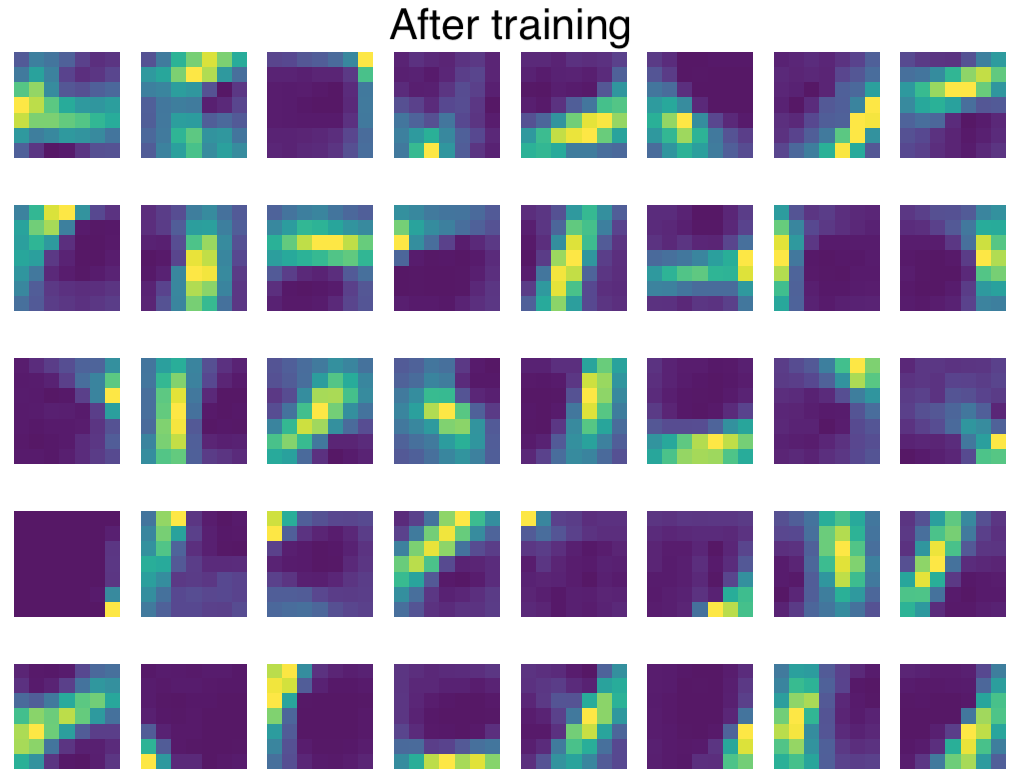
\includegraphics[width=12cm]{predictive_coding_stacked2_experiment3 after}
	\caption{Receptive fields of 20 neurons from a single column in layer 3 before and after training.}
	\label{fig:experiment3}
\end{figure} 
 


\section{Reinforcement learning and control}

\iffalse
The current dominant view of the brain has been heavily focused on optimisation.
All existing models of neural networks revolve around the idea that there exists some hidden error function that needs to be minimised. In reality there is nothing about the brain that resembles optimisation. Instead of fitting data, its fundamental principle is to build models of the world. In ECC networks, every single neuron tries to capture certain specific phenomenon of the external world. Every neuron is its own model. Perhaps we could summarise this idea as ``billion brains theory'', because we have billions of neurons and each one of them encodes some idea. The consciousness itself is decentralised. You can never lose your consciousness in its entirety. If your fusiform face area is damaged, you will lose the part of your consciousness that holds models of faces. If your hippocampus is removed, you will lose a fragment of consciousness that holds your recent memories.  In this view, every single neuron behaves like a miniature brain in and of itself. If $\boldsymbol{x}$ encodes the outside world, then each $y_i$ represents some tiny fragment of it. As you increase the number of neurons $\boldsymbol{y}$, you subdivide the world into billions of small interdependent ideas $p(\boldsymbol{x})=p(\boldsymbol{x},a_1)+...+p(\boldsymbol{x},a_{10^9})$.
\fi

The deep neural networks learn using backpropagation. They are inherently a supervised method of building intelligence. Even when the labels and error comes from the data itself, in a self-supervised manner, the learning still relies on the same supervised mechanisms. Deep nets can be applied to reinforcement learning problems by modelling the reward function. ECC networks on the other hand are purely unsupervised. They can't represent policy or reward function in any meaningful way. However, the biological brains are capable of performing control tasks very well. How could we achieve the same using ECC networks?


Reinforcement learning can be reformulated in a purely unsupervised way via introduction of energy $E$. The reward is defined as the derivative of energy, with respect to time
\[
R(t) = \frac{dE}{dt}
\]
When the agent finds source of energy, it will receive the feeling of reward.
Movement and action require energy. Even remaining idle will slowly lead to depletion of its reserves. This is the reason why animals tend to choose straight-line paths towards their destinations. 

The exploration and exploitation dilemma can be solved very elegantly. The energy is intrinsic to the agent. It will always know exactly how much it has and if the agent feels like it has access to abundant reserves of energy it could then decide to waste some of it by freely foraging and exploring. We can introduce a ``hunger'' constant  $h$. If $E<h$ then agent performs exploitation, otherwise it undertakes exploration.

The integral of $R$ is equivalent to sum of future rewards $R$, also commonly known as the return $G$. This is equal to the energy at some future time $E(T)$
\[
\int_{t=now}^{T} R dt = G(T) - G(now) = E(T)
\]
Suppose that sources of energy are scarce in the environment. Then finding any source of energy already has high probability of maximising the reward. Therefore we do not need to be preoccupied too much with ``maximising'' and should instead focus on ``finding'' anything at all. 

The agent never receives any reward. It doesn't actually exist. The reward is only something abstract and visible to an external observer, but internally the ECC networks have no concept of reward . This is the key difference between supervised and unsupervised reinforcement learning (figure \ref{fig:rl}). There is no reward. Instead, the network learns by modelling its effective fields. In order to define what this means, we need to assume that the agent is embodied. Let $\boldsymbol{u}$ be a binary vector representing motor neurons.
Analogically to receptive fields $p(\boldsymbol{x}|y_j)$ modelling input, the effective field
$p(\boldsymbol{u}|y_j)$ is a model of output. This is the probability that certain pattern of motor neurons activates in response to $y_j$ firing. The $\boldsymbol{y}$ neurons do not know their effective fields, hence feedback input $\boldsymbol{f}$ is necessary. It's a special type of input that carries back information about the action performed by $\boldsymbol{u}$. The receptive field $p(\boldsymbol{f}|y_j)$ works as a proxy for learning effective fields $p(\boldsymbol{u}|y_j)$. In very simple networks, both $\boldsymbol{u}$ and $\boldsymbol{f}$ might be coded using the same population of neurons, but in more complex topologies this may not be the case. Similarly we could think of $\boldsymbol{f}$ as a subpopulation of $\boldsymbol{x}$. 

The agent has two modelling tasks, both unsupervised. One of them is learning to anticipate $\boldsymbol{x}$ and $\boldsymbol{f}$ in the next time-step, knowing the current output $\boldsymbol{u}$. The second task involves planning and it tries to model the right output $\boldsymbol{u}$ that leads to the desired (distant) future internal state $E$ and $\boldsymbol{y}$. The neurons $\boldsymbol{y}$ build an internal model of the outside world and they compete for control over $\boldsymbol{u}$, similarly to how inputs $\boldsymbol{x}$ ``compete'' to trigger changes in $\boldsymbol{y}$.

\begin{figure}[!htbp]
	\centering
	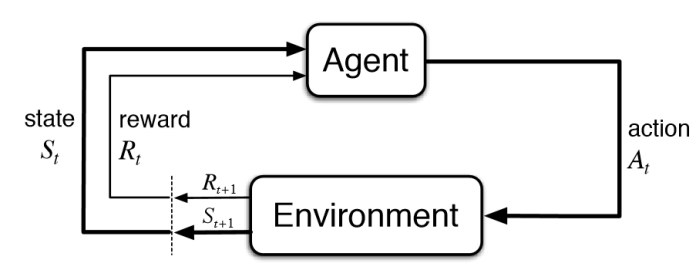
\includegraphics[width=10cm]{supervised reinforcement learning}
	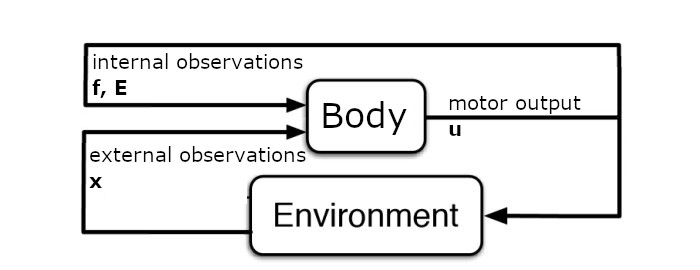
\includegraphics[width=10cm]{unsupervised reinforcement learning}
	\caption{Comparison of supervised (top) and unsupervised (bottom) reinforcement learning}
	\label{fig:rl}
\end{figure} 

If the agent builds an internal model of the world, that works like a map, it could then use such cognitive map to very quickly and efficiently search for energy sources. This only requires imagination, which is much cheaper than locomotion. The ECC networks do not see any reward. Instead, when the energy increases, certain neurons become temporarily more plastic than usually. This mechanism could be used to bias the cognitive map more towards places and actions that lead to the source of energy.

Once the agent has an internal map, it could then exactly know which aspects of the environment are unexplored. Unlike in the current deep reinforcement learning approaches, an agent with episodic memory would only need to visit a novel place once in order to learn about it. If the world is dynamically changing, then an attention mechanism will be necessary. If an animal sees or hears something unexpected it will focus all its attention on the novel experience. This mechanism can be explained using ECC networks as well. Suppose that the current internal model $\boldsymbol{y}$ explains all the previously experienced observations $p(\boldsymbol{x})=\sum_j p(\boldsymbol{x},y_j)$. If the agent experiences something novel that does not fit into any specific $y$, then it will be surprised. The agent will become curious and focus on the novel experience for a while. After the model  $\boldsymbol{y}$ restructures itself and learns about the new $\boldsymbol{x}$, then the agent become ``bored''. 



\section{Time and feedback (bonus)}

The ECC can be extended to work with time series, model sequential data, detect movement and distance of object. Let $\boldsymbol{x}^{(t)}$ and $\boldsymbol{y}^{(t)}$ be the input signal and states of neurons at time step $t$ respectively. We can concatenate several such vectors $\boldsymbol{x}^{(t-b)}\cdot \boldsymbol{x}^{(t-b+1) }\cdot ...\cdot\boldsymbol{x}^{(t)}=\boldsymbol{\hat{x}}^{(t)}$ up to $b$ steps from the past. Analogically for $\boldsymbol{\hat{y}}^{(t)}$. Now the weight matrices $W$ can span not only neurons but also their past states. The connections are now made not only across space but also time. This mechanism works identically in both discrete and continuous time. The dendrites of real neurons in the brain carry their information at different speeds. The faster dendrites connect to recent past, whereas slower ones detect signal from to more distant past. Aside from increased complexity, all the fundamental mechanism of ECC networks remain the same.

Every neuron represents certain aspect of the external world. Inhibitory neurons can be used to model logical negations, whereas excitatory neurons detect conjunctions. Sometimes it might be beneficial to model logical implications or equivalences. Figure \ref{fig:implication} 
\begin{figure}[!htbp]
	\centering
	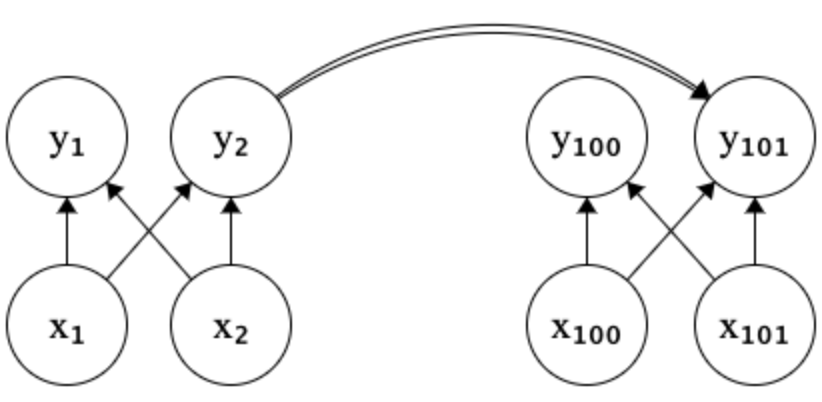
\includegraphics[width=10cm]{implication}
	\caption{Two distant columns connected by long range apical feedback}
	\label{fig:implication}
\end{figure} 
presents an example of two very distinct columns of neurons. Their topological receptive fields might be unrelated (for example one getting input from vision and the other from audition). The double arrow connecting $y_2$ to $y_{101}$ is used to denote that $y_{101}$ is only allowed to fire if  $y_2$ has previously fired. This way we can encode logical implication $y_{101} \implies y_{2}$. Connections like this are commonly observed in the real brain. The pyramidal neurons have two integration zones and will fire only when both are active at the same time. Such feedback allows for building network topologies that restrict the patterns of activities in certain specific ways and detect coincidences across different modalities.

\section{Optimisation (bonus)}

Sparsity enables major optimisations. We can define ECC layers with thousands of neurons, leading to $W$ matrices with millions of weights. Computing them is cheap and can be done on a single CPU because the input vector is sparse and binary. We do not need to multiply $\boldsymbol{x}W$ entirely. If we represent $\boldsymbol{x}$ as a list of indices of active neurons, then we can only iterate such list and visit only a handful of columns in $W$. The $argmax$ operation is linear. We can also implement $top-k$ algorithm with linear complexity, because the upper bound on $s$ is known in advance and we can use an approach similar to radix sort. During learning we have to renormalise the winning column of $W$. This requires computing sum, which is of linear complexity. We can achieve constant complexity if we implement a stochastic algorithm, that is, we add $\epsilon$ to $w_{ik}$ for $x_i=1$ (this operation is constant because $\boldsymbol{x}$ is sparse) and then we randomly choose a few other $w_{ik}$ for $x_i=0$ and subtract $\epsilon$ from them. We might need to check if $w_{ik}>0$ in order to avoid introducing negative values. This ensures that weights always sum up to $1$.

The real brain can function on a few potatoes a day. With neuromorphic hardware, ECC networks should be able to do the same. In theory we could have human-level intelligence running on cheap small chips. It's hard to imagine what a supercomputer could achieve.

We ran benchmarks on random patches of MNIST images. Each patch was 25x25 pixels. The network had 734400 learnable parameters (and several non-learnable sparse matrices). Our implementation written in Rust was able to process 2000 images per second on a single thread on 2.7 GHz Intel i5 core. When learning was enabled, it could train on 1700 images per second.

\section{Place cells (bonus)}

The experimental results above only present formation of receptive fields. If we wanted to solve MNIST, we would need to find a way of extracting outputs from ECC networks. This can be done using a binding mechanism. 
Suppose that there is an ECC network with several layer and the top one produces a collection of features describing certain observation. We would like to cluster those bags of features into categories. Suppose we generate a set of layers, one per category. We choose one of them and put it on top of our existing architecture. Then we present several example belonging to that specific category and let the network learn. Then we swap the top layer for a different one and draw examples from its corresponding category. After all learning is done, we concatenate all of the new layers into one and put it on top of the architecture. Now whenever a new examples comes our way, we will classify it into the category that receives the most votes.

Figure \ref{fig:v3 experiment2} presents results of training on full MNIST images. It can be seen that each neuron attends to a specific sub-feature of a digit. Several unrelated digits may share common features. For example a straight tilted line in the middle might code part of number $7$ or $4$. We finding $top-k$ neurons and combining their features we can narrow-down a specific digit. The distribution of observation vectors $p(\boldsymbol{x})$ might be very complex and we could approximate it well using millions of exclusive classes 
\[
p(\boldsymbol{x})=\sum_{j=1}^{10^6}p(\boldsymbol{x},z_j)
\]
This approach is wasteful, because very often several of the classes might share common features. For example we could approximate one $z$ using combination of  simpler ones from an intermediate layer $\boldsymbol{y}$ 
\[
p(\boldsymbol{x},z_3) = p(\boldsymbol{x},y_{54}) + p(\boldsymbol{x},y_{13}) + p(\boldsymbol{x},y_{183})
\] 
Learning using conjunctions of features is much cheaper and more robust than trying to overfit every single observation. We only need a device that could very quickly reuse and recombine features. In the real brain this is done by the hippocampus. It is the mechanism that effectively allows for one-shot learning.
Our implementation of the hippocampal-like ``place cells'' achieves 97\%+ accuracy on MNIST after seeing only a handful of examples (Figure \ref{mnist_results}). Certain pretraining is necessary in order to develop the smaller features, but it could be done even on unrelated data.

\begin{figure}[!htbp]
	\centering
	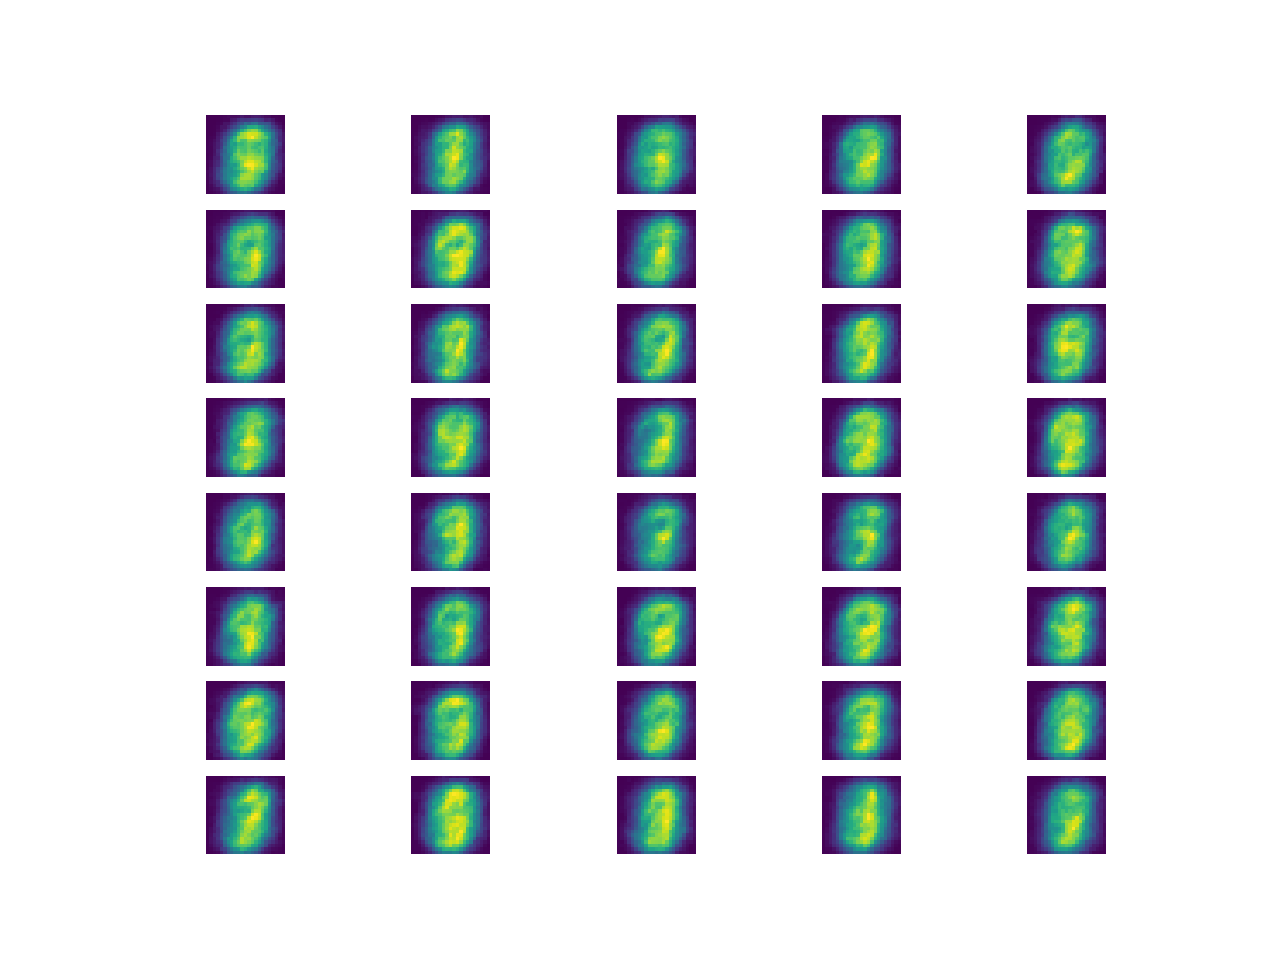
\includegraphics[width=10cm]{predictive_coding_stacked3_experiment2 before}
	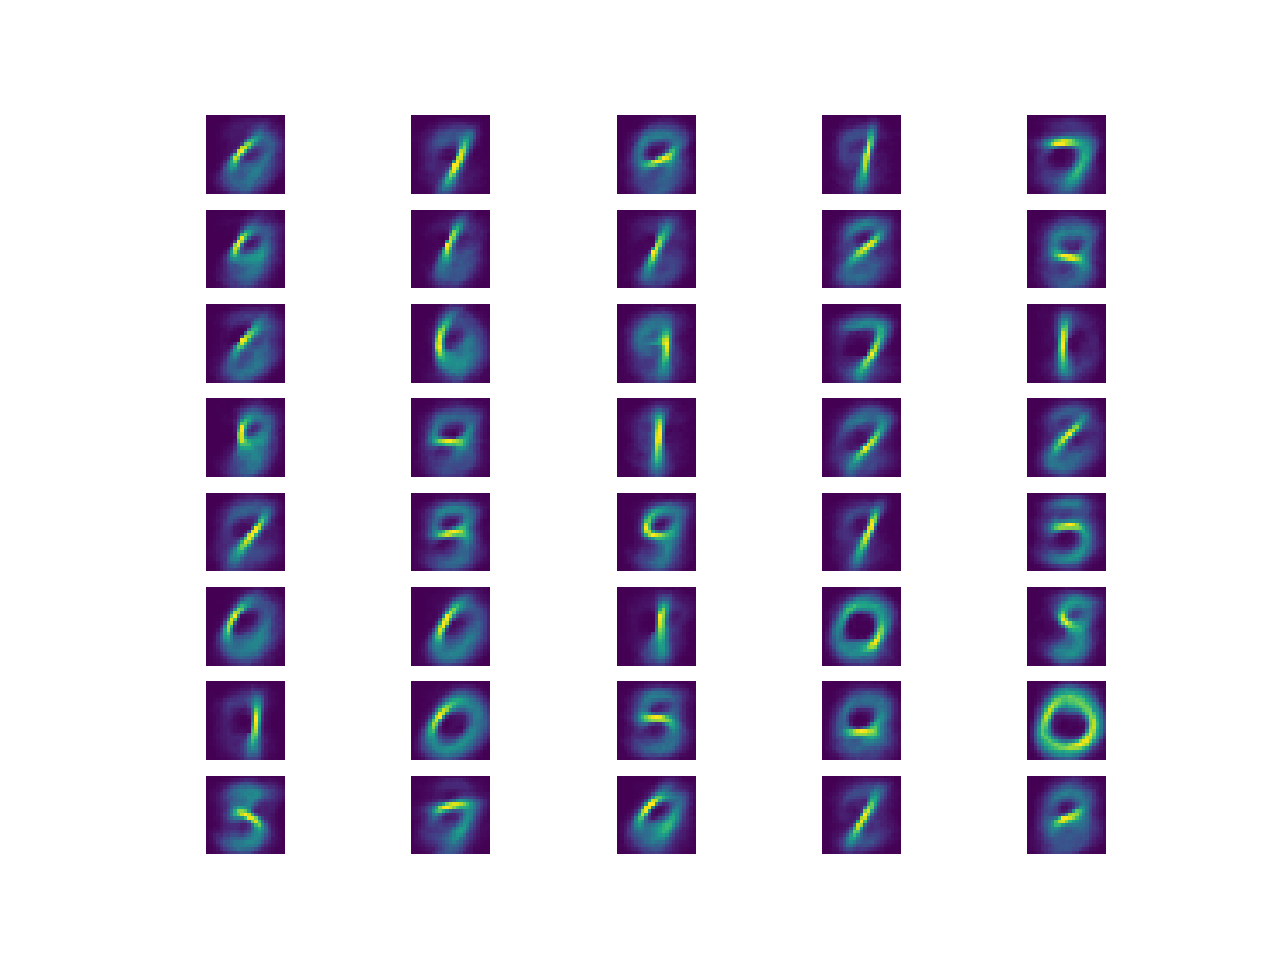
\includegraphics[width=10cm]{predictive_coding_stacked3_experiment2 after}
	\caption{Sub-features emerging in layer 5}
	\label{fig:v3 experiment2}
\end{figure} 

\section{Grid cells (bonus)}

The brain receives two types of experiences. Sensory input encode the state of the outside world. Motor feedback encodes the actions and state of the agent itself. What would happen if a neuron's receptive field included both types of information?
It leads to emergence of neurons that encode the state of the agent. Head-direction cells tell us which way we are facing. Grid cells encode our current location. 
Signals from such neurons can later be used to drive evolution of place cells.
Below we present an ECC architecture that leads to emergence of sensorimotor control. It enables the agent to anticipate outcomes of its actions. We show that it 
robustly and precisely predicts evolution of an interactive system over time.


\section{Invariance (bonus)}

The ECC do not need to share weights in the same way as deep neural nets do.
We could impose invariance by choosing the right connection topologies instead.
A grid-like lamellar pattern could be used for such a purpose. Suppose we are working in 3D space. Imagine a band of parallel axons running along $xz$ plane (perpendicular to $y$ axis). All axons are directed from positive $x$ to negative $x$ and run parallel to $x$ axis. If you now run a dendrite along the $z$ axis right on top of the band of axons, you will achieve topology, which connects that dendrite to every axon on that specific height. You can repeat this construction at different heights $y$. It doesn't matter which axon fires along the $z$ axis, but the height $y$ makes a difference. Hence the network topology is invariant to the dimension $z$ but sensitive to $y$. Different output neurons reside at distinct $x$ positions.

Structures like this have been observed in dentate gyrus of the hippocampal formation. We do not present any evidence that this is the purpose of lamellar structure of dentate gyrus, but we merely point out that it's a possibility and it could be imitated by ECC networks.

\section{Planning (bonus)}

By mimicking the mechanisms of hippocampal formation, we can design ECC networks capable of imagination and forward thinking. Perhaps by building on top of it, we could reproduce higher cognitive functions of prefrontal cortex but this is beyond the scope of this paper. Figure \ref{fig:hippocampus} presents three layers arranged in a loop.
\begin{figure}[!htbp]
	\centering
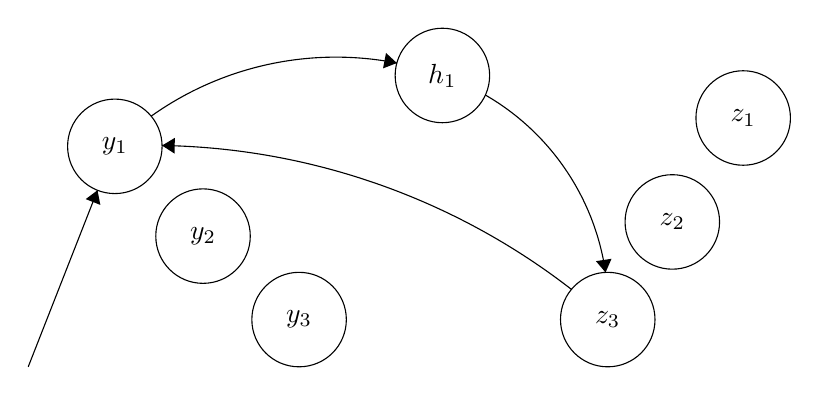
\begin{tikzpicture}[scale=0.2]
	\tikzstyle{every node}+=[inner sep=0pt]
	\draw [black] (22.6,-31.5) circle (3);
	\draw (22.6,-31.5) node {$y_1$};
	\draw [black] (28.2,-37.2) circle (3);
	\draw (28.2,-37.2) node {$y_2$};
	\draw [black] (34.3,-42.5) circle (3);
	\draw (34.3,-42.5) node {$y_3$};
	\draw [black] (43.4,-27) circle (3);
	\draw (43.4,-27) node {$h_1$};
	\draw [black] (53.9,-42.5) circle (3);
	\draw (53.9,-42.5) node {$z_3$};
	\draw [black] (58,-36.3) circle (3);
	\draw (58,-36.3) node {$z_2$};
	\draw [black] (62.5,-29.7) circle (3);
	\draw (62.5,-29.7) node {$z_1$};
	\draw [black] (24.906,-29.585) arc (125.45796:78.9572:20.22);
	\fill [black] (40.51,-26.21) -- (39.82,-25.57) -- (39.63,-26.55);
	\draw [black] (46.127,-28.24) arc (60.02539:8.20355:15.573);
	\fill [black] (53.76,-39.51) -- (54.14,-38.64) -- (53.15,-38.79);
	\draw [black] (17.1,-45.5) -- (21.5,-34.29);
	\fill [black] (21.5,-34.29) -- (20.75,-34.85) -- (21.68,-35.22);
	\draw [black] (25.599,-31.446) arc (89.06231:52.2109:43.588);
	\fill [black] (25.6,-31.45) -- (26.39,-31.96) -- (26.41,-30.96);
\end{tikzpicture}
	\caption{Simplified schematic of hippocampal formation}
	\label{fig:hippocampus}
\end{figure} 
The neurons $\boldsymbol{y}$ receive input from lower levels of ECC network.
The layer $\boldsymbol{h}$ contains place cells (their activity is modulated by grid cells, which are not shown here). Suppose that the agent finds itself at a particular location and it sees some object. The representation of that experience will be encoded by $\boldsymbol{y}$ and this population activity will be associated to a particular populations of $\boldsymbol{h}$ cells. The $\boldsymbol{y}$  activity has only miniscule effect on activation of $h_1$ (it is mostly the grid cells that activate it, which function as a ``label'' for the inputs). The currently active $h_1$ drives activity in $\boldsymbol{z}$ layer (the subiculum in biological brains). The $z$ neurons have only a miniscule effect on activation of $\boldsymbol{y}$ layer. The plasticity of connections from $\boldsymbol{z}$ to $\boldsymbol{y}$ will learn to associate specific place cells with their most recent experiences (over time this will change and short-term memory will fade away). If the agent ``closes its eyes'' and there is no signal flowing to $\boldsymbol{y}$ from below, then $\boldsymbol{z}$ will be the sole force driving $\boldsymbol{y}$ activity. This allows for ``imagination''. Agent can use place cells $\boldsymbol{h}$ to imagine future experiences and relieve recent events. Sequences of such place cell activities have been observed in the real brain during planning. The mechanism above does not have enough storage capacity to keep long-term memories. There needs to exist a mechanism that transfers this information to other parts of the network (quite possibly during sleep they will be moved to prefrontal cortex and other areas).


\section{Evolving ECC networks (bonus)}

The receptive fields $p(\boldsymbol{x},y_j)$ of neurons are primarily driven by their respective topologies $\tau$. We can embed the set of all neurons $\boldsymbol{y}$ in a n-dimensional euclidean space. This way we obtain a norm on all nodes in the graph. Neurons that are in close proximity, should have higher probability of developing similar topologies. Then the task of evolving ECC network becomes reduced to evolution of manifolds in a euclidean space. Kenneth Stanley's ES-HyperNEAT algorithm can be repurposed for such a task. 

What should be the fitness function?  If we tried to evaluate ECC on CIFAR10, we would achieve seemingly poor results. That is because static data lacks any semantics and it's impossible to build meaningful models of the world when you all can see are shadows in Plato's cave. Hence it only makes real sense to evaluate ECC as reinforcement  learning agents. 

Should the accumulated reward be a fitness function? ECC networks lack any optimisation  mechanism and we are not sure whether there will even be any straight-forward way of precisely controlling agent's behaviour. If we couldn't explain to the agents exactly what they are supposed to do, then any measure of their ``success'' becomes vague and misleading. We believe that open-ended novelty search is the only reasonable approach. Hence there is no fitness function.

Developing AGI is going to be a creative process. We should experiment with various network topologies and investigate the receptive fields that they form. 
It would then be possible to build a zoo of interesting topologies and develop it like Picbreeder in a community-driven way. If we focus on finding interesting patterns, then it might be possible to build machines capable of feeling emotions, appreciating art and music, chasing mice like cats or dancing like peacock spiders.

% Even if humanity found a way of controlling the behaviour of ECC networks, we feel the need to make a grim warning against that. The last thing we need is to build AGI that is very good and collecting stamps but lacking any will to live or appreciation of the world.

% (My notes on the side: Interestingly, we don't know whether there exist other technologies capable of producing AGI, but if deep learning is one of them, then it seems like the right tool for building deadly emotionless killing machines. Hopefully deep learning never becomes truly intelligent. Paradoxically OpenAI's  and DeepMind's efforts towards achieving ``safe AGI'' have been only leading in the opposite direction.)


%\section{Evolving ECC networks (bonus)}
 
 %We can define an algebra of network topologies. Let $\mathbb{X}$ be the set of all neurons.



\bibliographystyle{BibTeXtran}   % (uses file "BibTeXtran.bst")
\bibliography{BibTeXrefs}    







\end{document}
